\subsection{Glyph: \glyph{Observable}}
\label{sec:af:observable}

A biochemical network can generate phenotypes or affect biological processes. Such processes can take place at different levels and are independent of the biochemical network itself. To represent these processes in a diagram, SBGN defines the observable glyph.

\begin{glyphDescription}

\glyphSboTerm SBO:0000358 ! observable

\glyphContainer An \glyph{observable} is represented by an elongated
hexagon, as illustrated in \fig{af:observable}.

\glyphLabel An \glyph{observable} is identified by a label placed in an
unbordered box containing a string of characters.  The characters can be
distributed on several lines to improve readability, although this is not
mandatory.  The label box must be attached to the center of the
\glyph{observable} container.  The label may spill outside of the container.

\end{glyphDescription}

\begin{figure}[H]
  \centering
  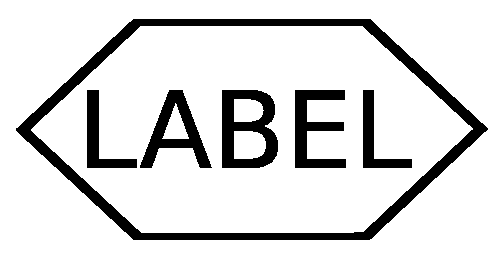
\includegraphics[scale = 0.3]{images/observable}
  \caption{The \AF glyph for \glyph{observable}.}
  \label{fig:af:observable}
\end{figure}
